
%version 2: \usepackage{hyperref}


%%%%%%%%%%%%%%%%%%%%%%%%%%%%%%%%%%%%%%%%%%%%%%%%%%%%%%%%%%%%%%%%%%%%%%%%
%Para las ecuaciones siempre es Ec.(n).
%Para las figuras siempre es Fig.n, incluso en el caption de la figura. Tambien las Tablas
%Para las referencias es [n]
%%%%%%%%%%%%%%%%%%%%%%%%%%%%%%%%%%%%%%%%%%%%%%%%%%%%%%%%%%%%%%%%%%%%%%%%

\documentclass[
reprint,
%notitlepage,
%superscriptaddress,
%groupedaddress,
%unsortedaddress,
%runinaddress,
%frontmatterverbose, 
%preprint,
%showpacs,preprintnumbers,
%nofootinbib,
%nobibnotes,
%bibnotes,
%11 pt,
amsmath,
amssymb,
%aps,
%pra,
prb,
%rmp,
%tightenlines %esto hizo el milagro de sacar los espacios en blancos estocásticos (?)
%prstab,
%prstper,
%floatfix,\textbf{}
]{revtex4-1} %Instalar primero para usarlo. Paquete malo.

%\documentclass[onecolumn, aps, amsmath,amssymb ]{article}
\usepackage{lipsum}  
\usepackage{graphicx}% Include figure files
\usepackage{subfig}
\usepackage{braket}
\usepackage{comment} %comment large chunks of text
\usepackage{dcolumn}% Align table columns on decimal point
\usepackage{bm}% bold math
%\usepackage{hyperref}% add hypertext capabilities
\usepackage[mathlines]{lineno}% Enable numbering of text and display math
%\linenumbers\relax % Commence numbering lines
\usepackage{mathtools} %% Para el supraíndice

\usepackage[nice]{nicefrac}

%%%%%%%El Señor Español%%%%%%%%%%%%%%%%%%%%%%%%%%%
\usepackage[utf8]{inputenc} %acento
\usepackage[
spanish, %El lenguaje.
es-tabla, %La tabla y no cuadro.
activeacute, %El acento.
es-nodecimaldot %Punto y no coma con separador de números
]{babel}
\usepackage{microtype} %para hacerlo más bonito :33 como vos (?) 
%%%%%%%%%%%%%%%%%%%%%%%%%%%%%%%%%%%%%%%%%%%%%%%%%%%
%%%%%%%%% Para que las imágenes se queden dónde las quiero (?
\usepackage{float}
%%%%%%%%%%
\usepackage{enumitem}
\usepackage{hyperref} % Para usar \url

%%%%%%%%Cambia a Fig de Figure%%%%%%%%%%
\makeatletter
\renewcommand{\fnum@figure}{Fig. \thefigure} 
\makeatother
%%%%%%%%%%%%%%%%%%%%%%%%%%%%%%%%%%%%%%%%
\raggedbottom

\usepackage{multirow}
\usepackage{paralist}
\begin{document}

\title{Práctica 6: Método basado en Árboles de Decisión}
\author{Evelyn G. Coronel}

\affiliation{Redes Neuronales y Aprendizaje Profundo para Visión Artificial\\ Instituto Balseiro\\}

\date[]{\lowercase{\today}} 

\maketitle

\section*{Ejercicio 1}

% (a)  Separar los datos en dos particiones, una para datos de entrenamiento/validación (osea, de desarrollo) y otra para test.

\subsection*{Item A}
Este ejercicio, se utilizan arboles de clasificación y regresión para obtener la cantidad de unidades de asientos para bebés se compran, en función de las características del producto y del lugar donde se venden. Las variables a tener en cuenta del conjunto de datos son:

\begin{compactenum}
	\item Sales: Cantidad de asientos vendidos en una tienda.
	\item CompPrice: Precio del asiento según la competencia.
	\item Income: Ingreso de dinero medio en miles de USD del lugar donde se localiza la tienda.
	\item Advertising: Inversión en propaganda de la tienda en  miles de USD.
	\item Population: Población local en miles.
	\item Price: Precio de venta por cada asiento.at each site
	\item ShelveLoc: Posición del asiento en vitrina, se clasifica las posición como Bad, Good and Medium  (Malo, Bueno y Medio).
	\item Age: Edad promedio de la población local.
	\item Education: Nivel de educación
	\item Urban: \emph{Yes} si la tienda está ubicada en un lugar urbano, \emph{No} caso contrario.
	\item US:\emph{Yes} si la tienda está ubicada en Estados Unidos, \emph{No} caso contrario.    
\end{compactenum}
Además de estas variables, se agregó una última variable llamada \emph{High} es \emph{Yes} si las ventas superan las $8$ unidades, \emph{No} caso contrario. 

Para realizar los ajustes, se transformaron los datos descriptos \emph{Yes} y \emph{No} como 1 y 0 respectivamente, y \emph{Good}, \emph{Medium}, \emph{Bad} con 3, 2 y 1. Además se separó el conjunto de datos en un $80\%$ de entrenamiento y un $20\%$ de validación. Las variables \emph{Sales} y \emph{High} se separan del resto de los atributos para hacer los ajustes.

% (b)  Entrenar un árbol de decisión para clasificación de la variableHigh. Hacer un plot delárbol (usarscikit-learn) e interpretar los resultados.
\subsection*{Item B}

Usando un árbol de decisión de clasificación, se utilizó la columna \emph{High} como salida esperada y el resto de los atributos como entrada. El árbol está instanciado de tal forma que  el ajuste se realice hasta que las hojas sean puras, es decir, que el coeficiente de gini del nodo sea 0. Con esto se obtuvo un árbol con las  características que se presentan en la Tabla~\ref{tab:item_B}. Los valores de precisión  son los scores para los datos de validación o entrenamiento según corresponda.

\begin{table}[H]
	\begin{small}
		\begin{center}
			\begin{tabular}[c]{l|l}
				Profundidad & 11 \\ \hline
				Hojas & 50 \\ \hline
				Error de entrenamiento & 0 de 320\\ \hline
				Precisión de entrenamiento & 1 \\ \hline
				Error de validación & 6 de 80\\ \hline
				Precisión de validación & 0.675 \\ 
			\end{tabular}
		\end{center}
	\end{small}
	\caption{Características del árbol de decisión de clasificación posterior al ajuste del item B}
	\label{tab:item_B}
\end{table}

Las primeras cuatro ramas del árbol se muestran en la Fig.\ref{fig:item_B_tree}. En este caso se llega hasta un profundidad de 11 porque no estamos limitando el valor de gini de las hojas, la clasificación  se realiza hasta que los datos de entrenamiento tengan una clasificación fiel, por eso se observa el overfitting del árbol. El primer nodo usa la posición en la vitrina  para clasificar los datos, ya que este parámetro divide mejor los datos, dicho de otra forma, tiene el coeficiente de gini mayor de todos los nodos.
\begin{figure}[H]
	\begin{small}
		\begin{center}
			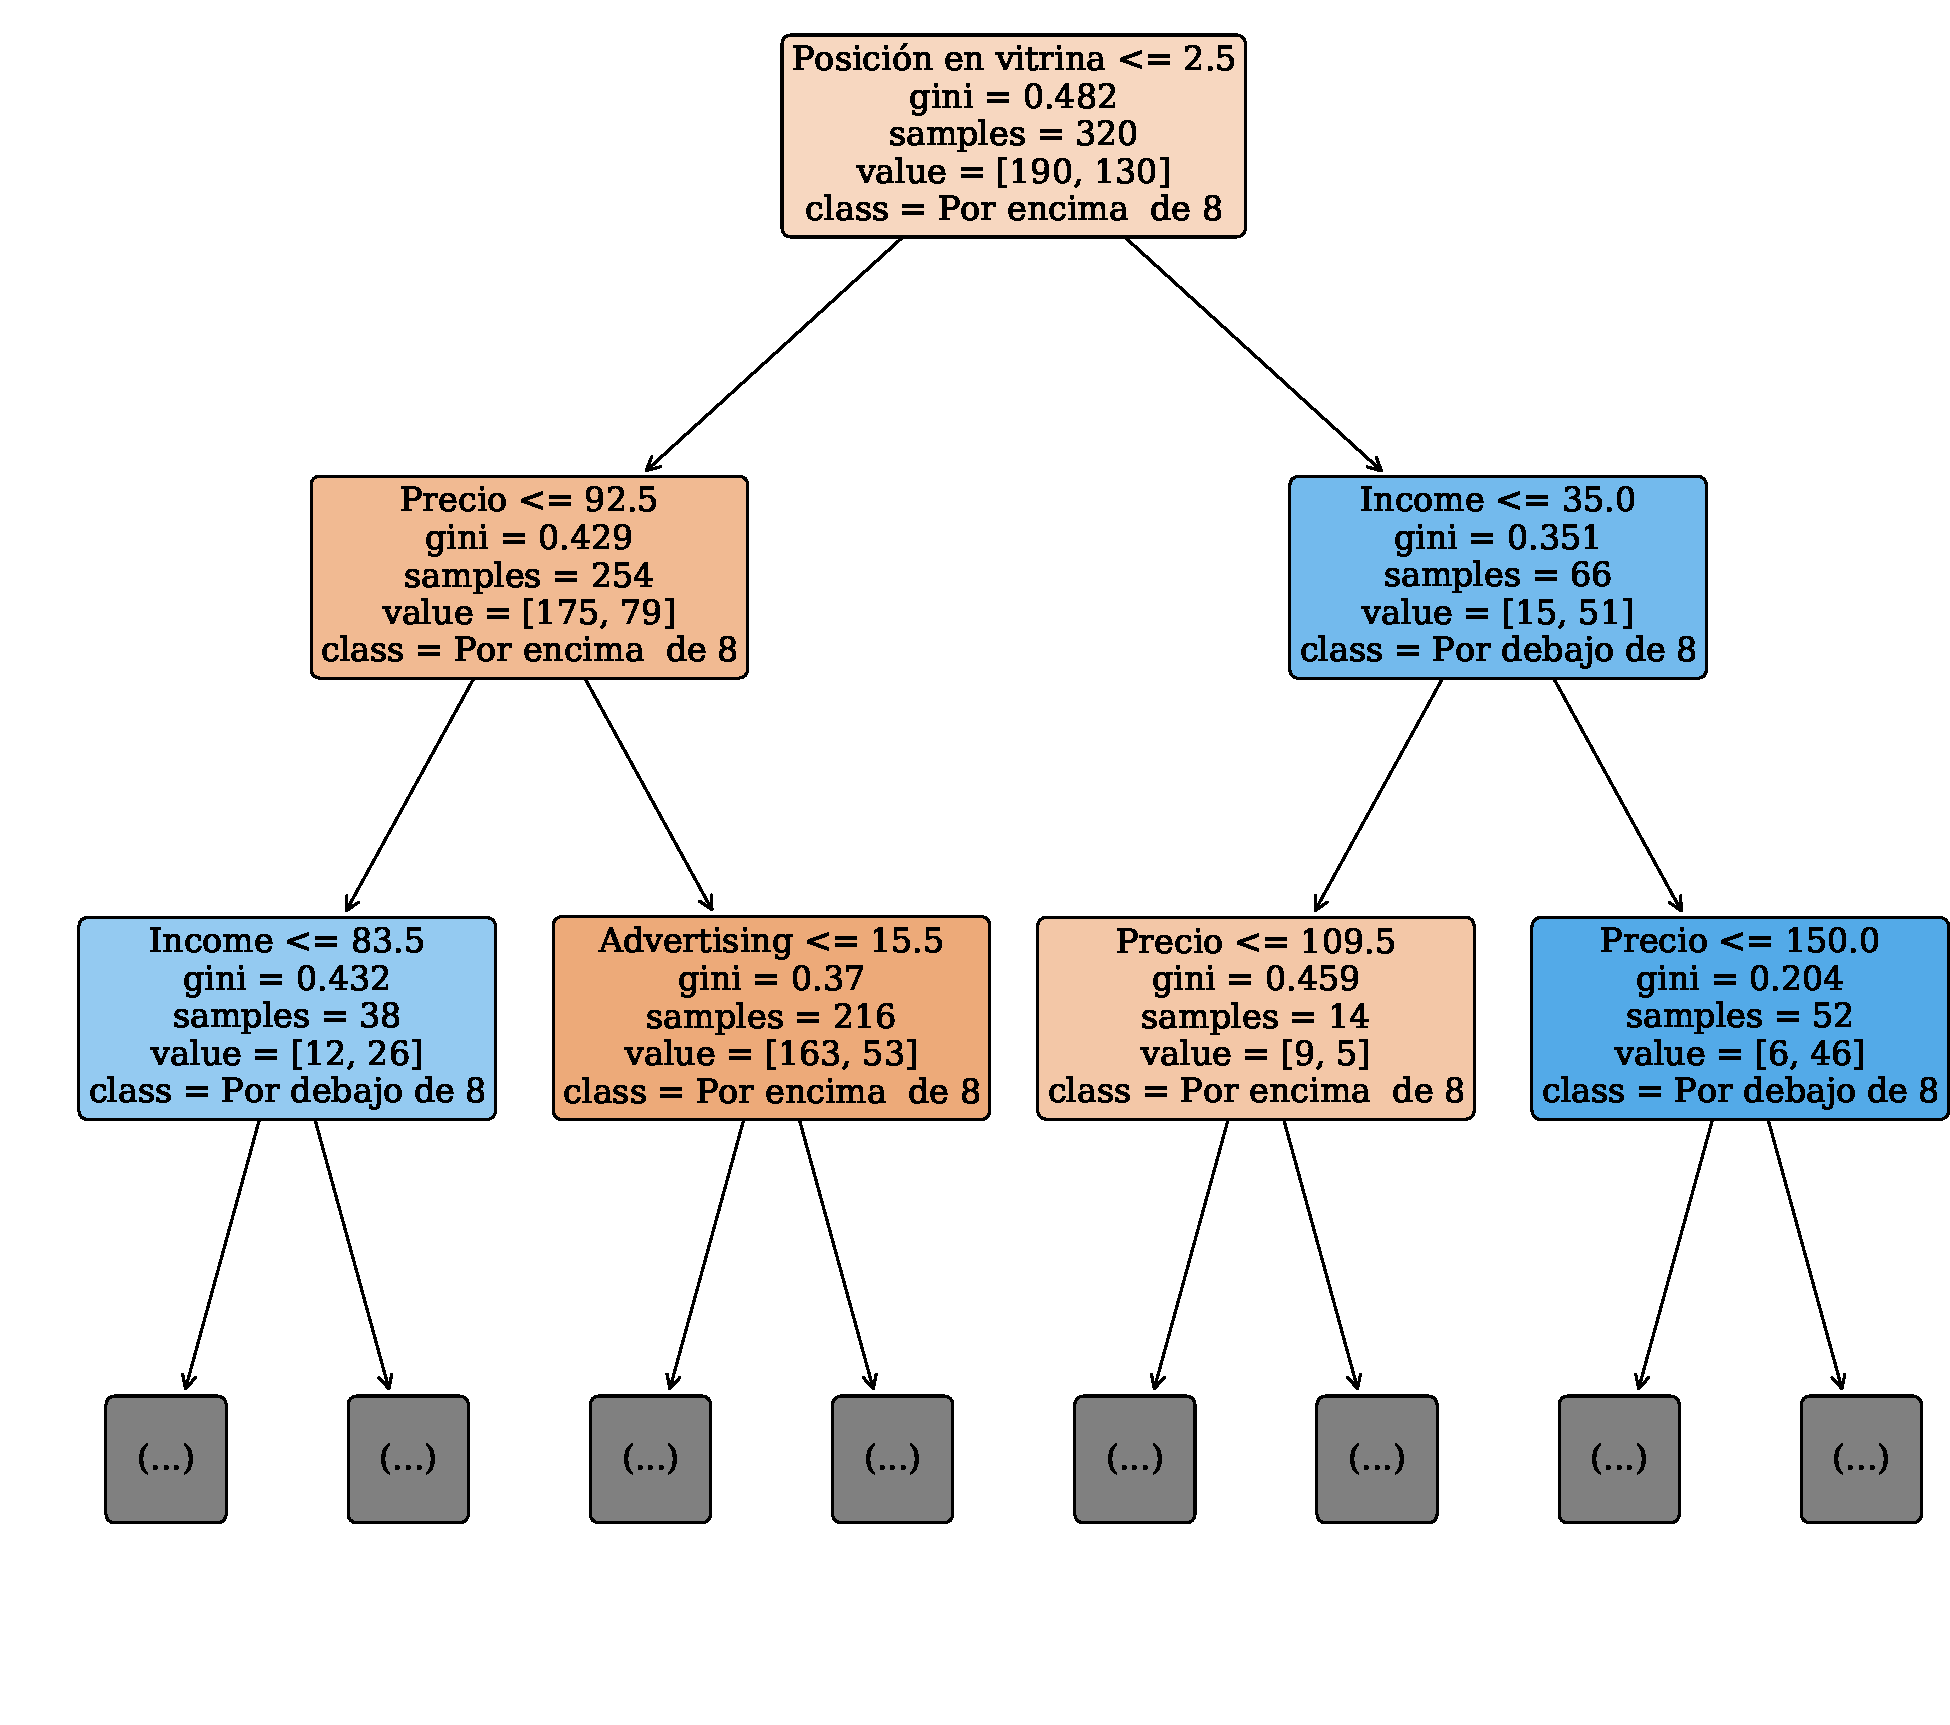
\includegraphics[clip,trim=0 4cm {.5\wd0} 0.5cm,width=0.5\textwidth]{figures/tree_B_tree.pdf}
		\end{center}
		\caption{Las primeras cuatro ramas de la estructura del árbol de clasificación para el item B.}
		\label{fig:item_B_tree}
	\end{small}
\end{figure}


% (c)  Entrenar un árbol de decisión para regresión de la variableSales.  Hacer un plot delárbol (usarscikit-learn) e interpretar los resultados.
\subsection*{Item C}

El árbol instanciado en este item es el árbol de regresión, los parámetros por defecto también hacen que el árbol regresione hasta tener hojas con gini nulo. Ahora los datos de salida esperado son los datos de la columna de \emph{Sales}. A partir de este item en adelante, el valor de error es el error cuadrático medio entre la salida predicha por el árbol y la salida esperada. Como se ven en la Tabla \ref{tab:item_C} se muestran las características del árbol luego de realizar el ajuste. Nuevamente se tiene un overfitting con el conjunto de entrenamiento. 
\begin{table}[H]
	\begin{small}
		\begin{center}
			\begin{tabular}[c]{l|l}
				Profundidad & 18 \\ \hline
				Hojas & 320 \\ \hline
				Error de entrenamiento & 0.0\\ \hline
				Precisión de entrenamiento & 1 \\ \hline
				Error de validación & 0.073\\ \hline
				Precisión de validación & 0.247 \\ 
			\end{tabular}
		\end{center}
	\end{small}
	\caption{Características del árbol de regresión posterior al ajuste en el item C}
	\label{tab:item_C}
\end{table}
\begin{figure}[H]
	\begin{small}
		\begin{center}
			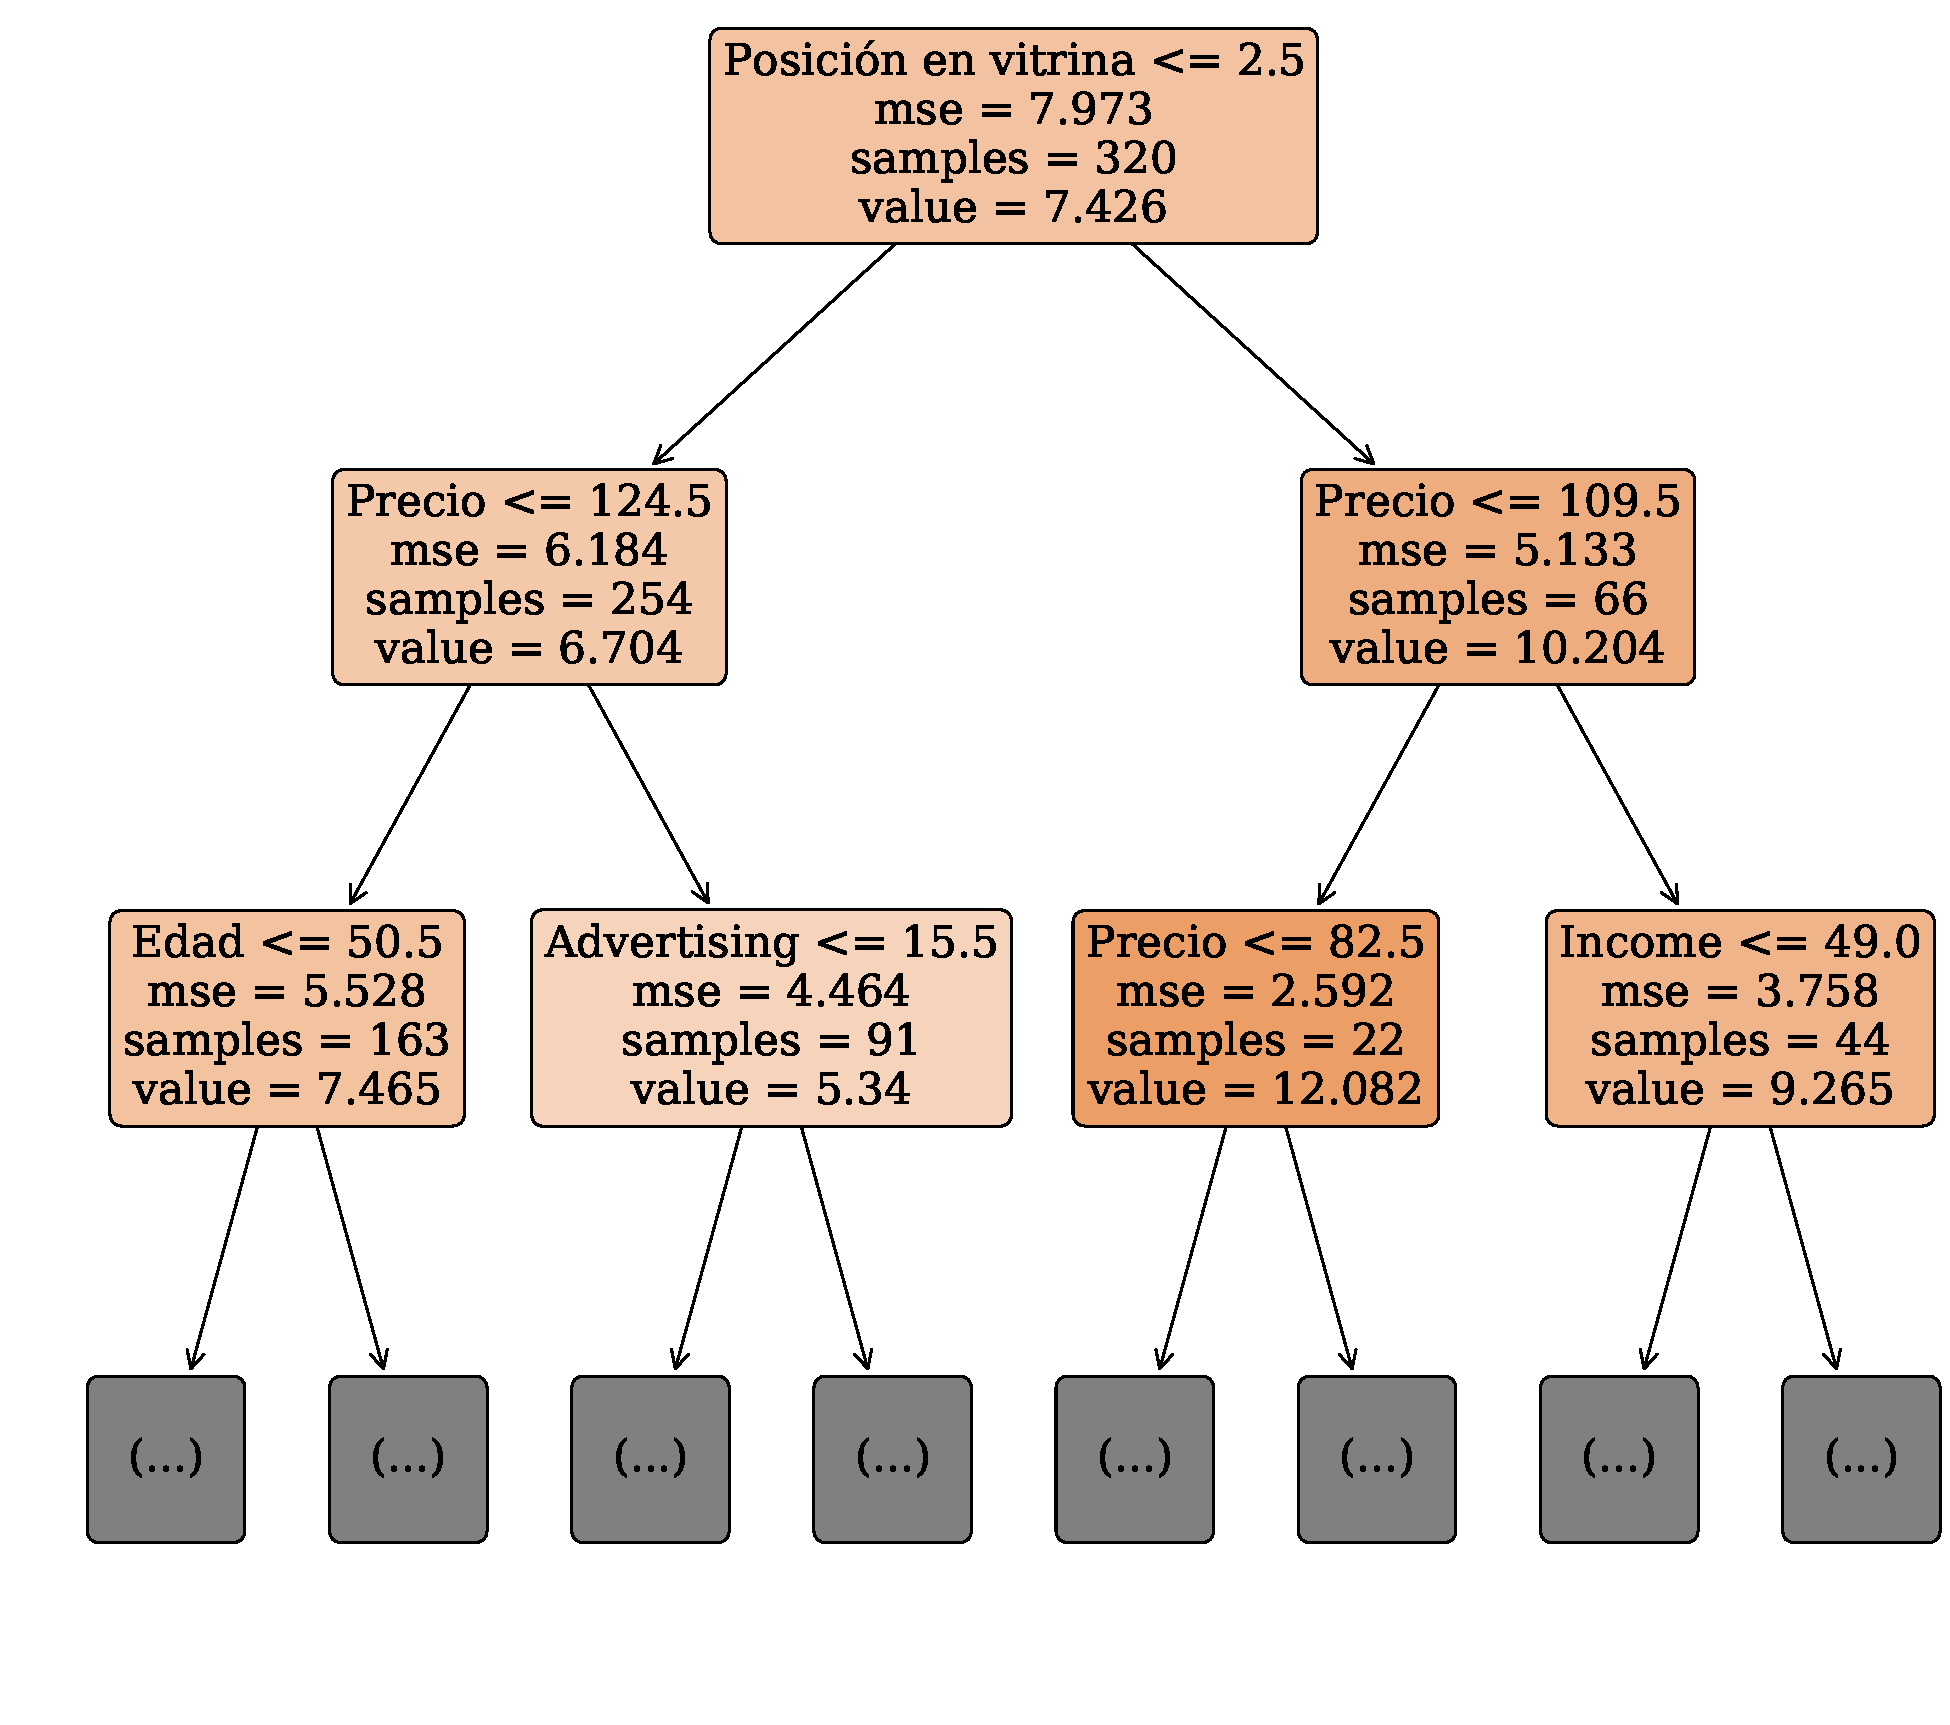
\includegraphics[clip,trim=0 3.8cm {.5\wd0} 0, width=0.5\textwidth]{figures/tree_C_tree.pdf}
		\end{center}
		\caption{Las primeras cuatro ramas de la estructura del árbol de clasificación para el item C.}
		\label{fig:item_C_tree}
	\end{small}
\end{figure}

A pesar del overfitting del árbol, el árbol aprende la correlación de los atributos con la cantidad de asientos. Esto se observa en la Fig.\ref{fig:item_C_scatter}, dado que los ejes x e y son la cantidad de asientos reales y predichos, mientras más cerca estén los puntos a la línea, mejor es la predicción del árbol.

% (d)  ¿Cuál es el error de test que obtienen en cada caso?  Comparar con el error de entrenamiento y determinar si tienen overfitting o no.
\subsection*{Item E}

% (e)  Para el árbol de regresión, usarcross-validationpara determinar el nivel óptimo de com-plejidad del árbol.  Busquen cómo usar enscikit-learnla técnica depruningparamejorar la tasa de error de test.

En este ejercicio se utilizó  la función  \verb|GridSearchCV|, que toma vectores con valores para los parámetros de profundidad del árbol \verb|max_depth| y el coeficiente de  \emph{Cost-Complexity Pruning}. Este último impone un valor mínimo para el cual el nodo se considera una hoja o no, disminuyendo así el overfitting del árbol. 
\begin{figure}[H]
	\begin{small}
		\begin{center}
			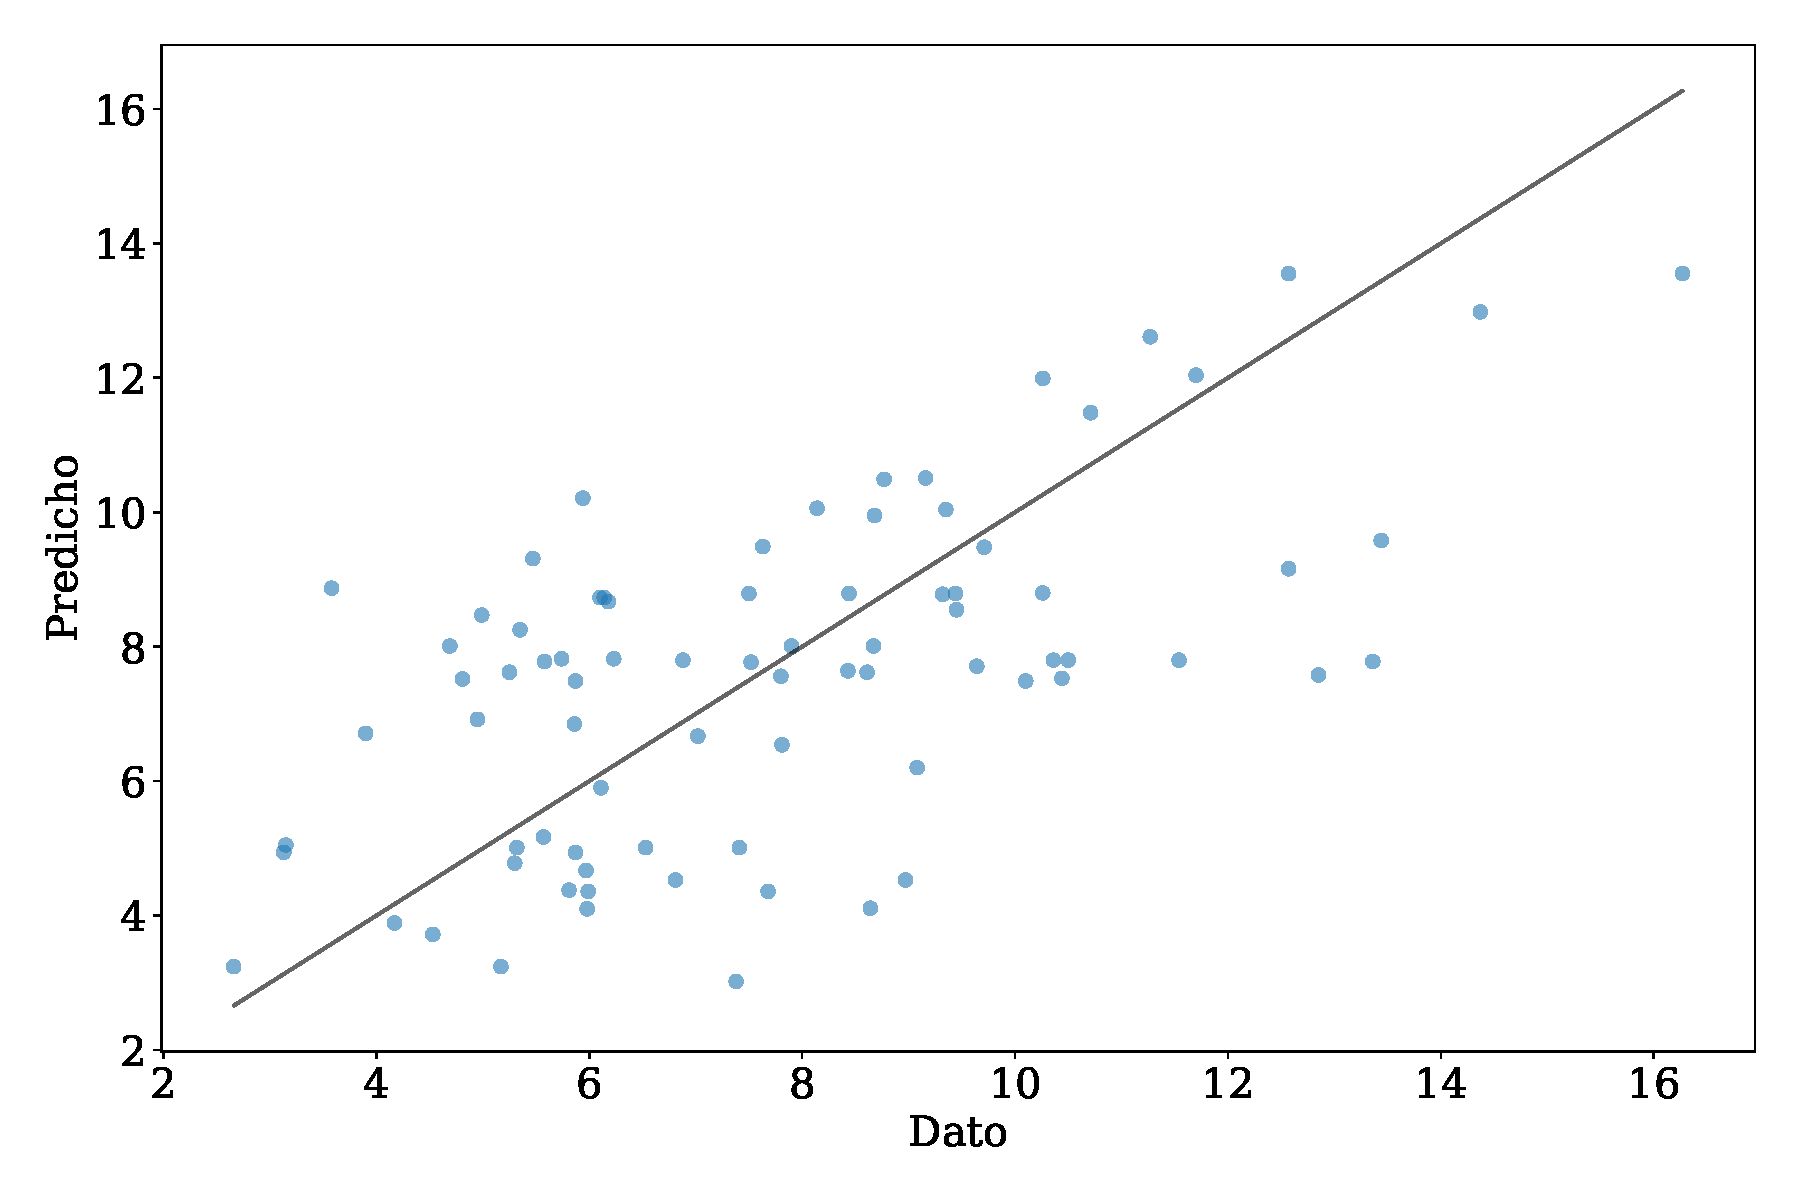
\includegraphics[width=0.45\textwidth]{figures/fit_C_tree.pdf}
		\end{center}
		\caption{Comparación entre el dato y la predicción del árbol de regresión para else item C.}
		\label{fig:item_C_scatter}
	\end{small}
\end{figure}

Mediante la función \verb|GridSearchCV|, se calculan los parámetros que maximizan el \emph{score} mediante k-fold \emph{cross validation}(CV). La función tiene un valor predeterminado de $k=5$ que fue el utilizado.

Los parámetros óptimos obtenidos son: Profundidad igual a $5$ y coeficiente de  \emph{Cost-Complexity Pruning} ó $\alpha_{ccp}$ igual a $0.2$, donde el mejor  score obtenido  fue de $0.36$. Posterior al entrenamiento con estos parámetros, el árbol tiene las características listadas en la Tabla \ref{tab:item_E}. Ahora el error de validación para este item es menor que el item B, donde  de $0.07$ pasa a $0.06$, pero la precisión sobre los datos de validación es mayor en el  caso anterior. La Fig.\ref{fig:item_E_scatter} muestra la comparación entre precio predicho y real, en el mismo se que los precios predichos sigue la tendencia de los reales, a pesar de la baja precisión.

\begin{table}[H]
	\begin{small}
		\begin{center}
			\begin{tabular}[c]{l|l}
				Profundidad & 5 \\ \hline
				Hojas & 10 \\ \hline
				Error de entrenamiento & 0.009\\ \hline
				Precisión de entrenamiento & 0.60 \\ \hline
				Error de validación & 0.06\\ \hline
				Precisión de validación & 0.35 \\
			\end{tabular}
		\end{center}
	\end{small}
	\caption{Características del árbol de regresión posterior al ajuste en el item E}
	\label{tab:item_E}
\end{table}


Además de la función \verb|GridSearchCV|, se utilizó el método \verb|cost_complexity_pruning_path| propia de la clase \verb|DecisionTreeRegressor|, que devuelve los valores posibles de $\alpha_{cpp}$. Con los mismos se calcularon los errores  y profundidades a las que llega los datos de entrenamiento, y el error de  los datos de validación. En la Fig.\ref{fig:params_ccp} se muestra como varian los errores y la profundidad con $\alpha_{cpp}$ y se observa un mínimo en el error de validación para un valor de $\alpha_{cpp}=0.25$, donde la red tiene una profundidad de 5 niveles.

\begin{figure}[H]
	\begin{small}
		\begin{center}
			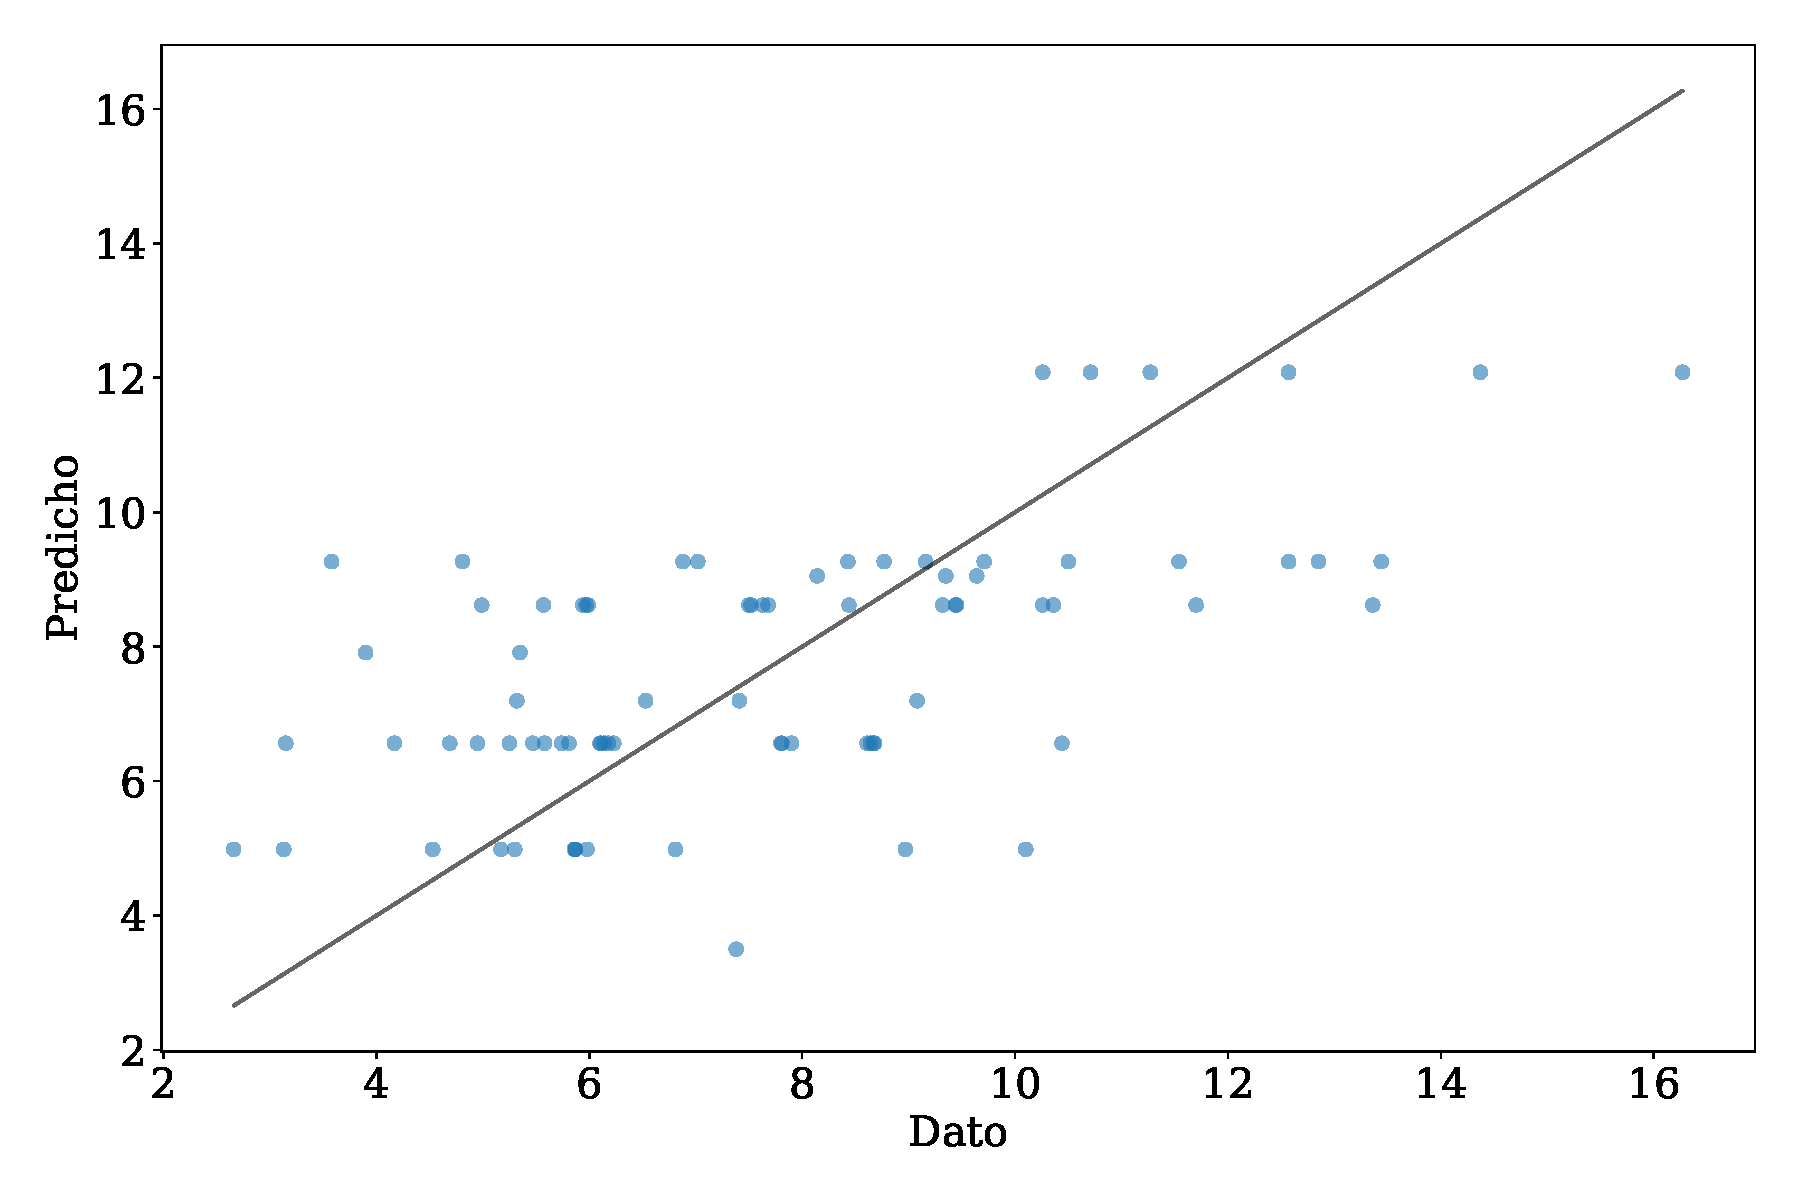
\includegraphics[width=0.45\textwidth]{figures/fit_E_tree_optimo.pdf}
		\end{center}
		\caption{Comparación entre el dato y la predicción del árbol de regresión para el item E.}
		\label{fig:item_E_scatter}
	\end{small}
\end{figure}
\begin{figure}[H]
	\begin{small}
		\begin{center}
			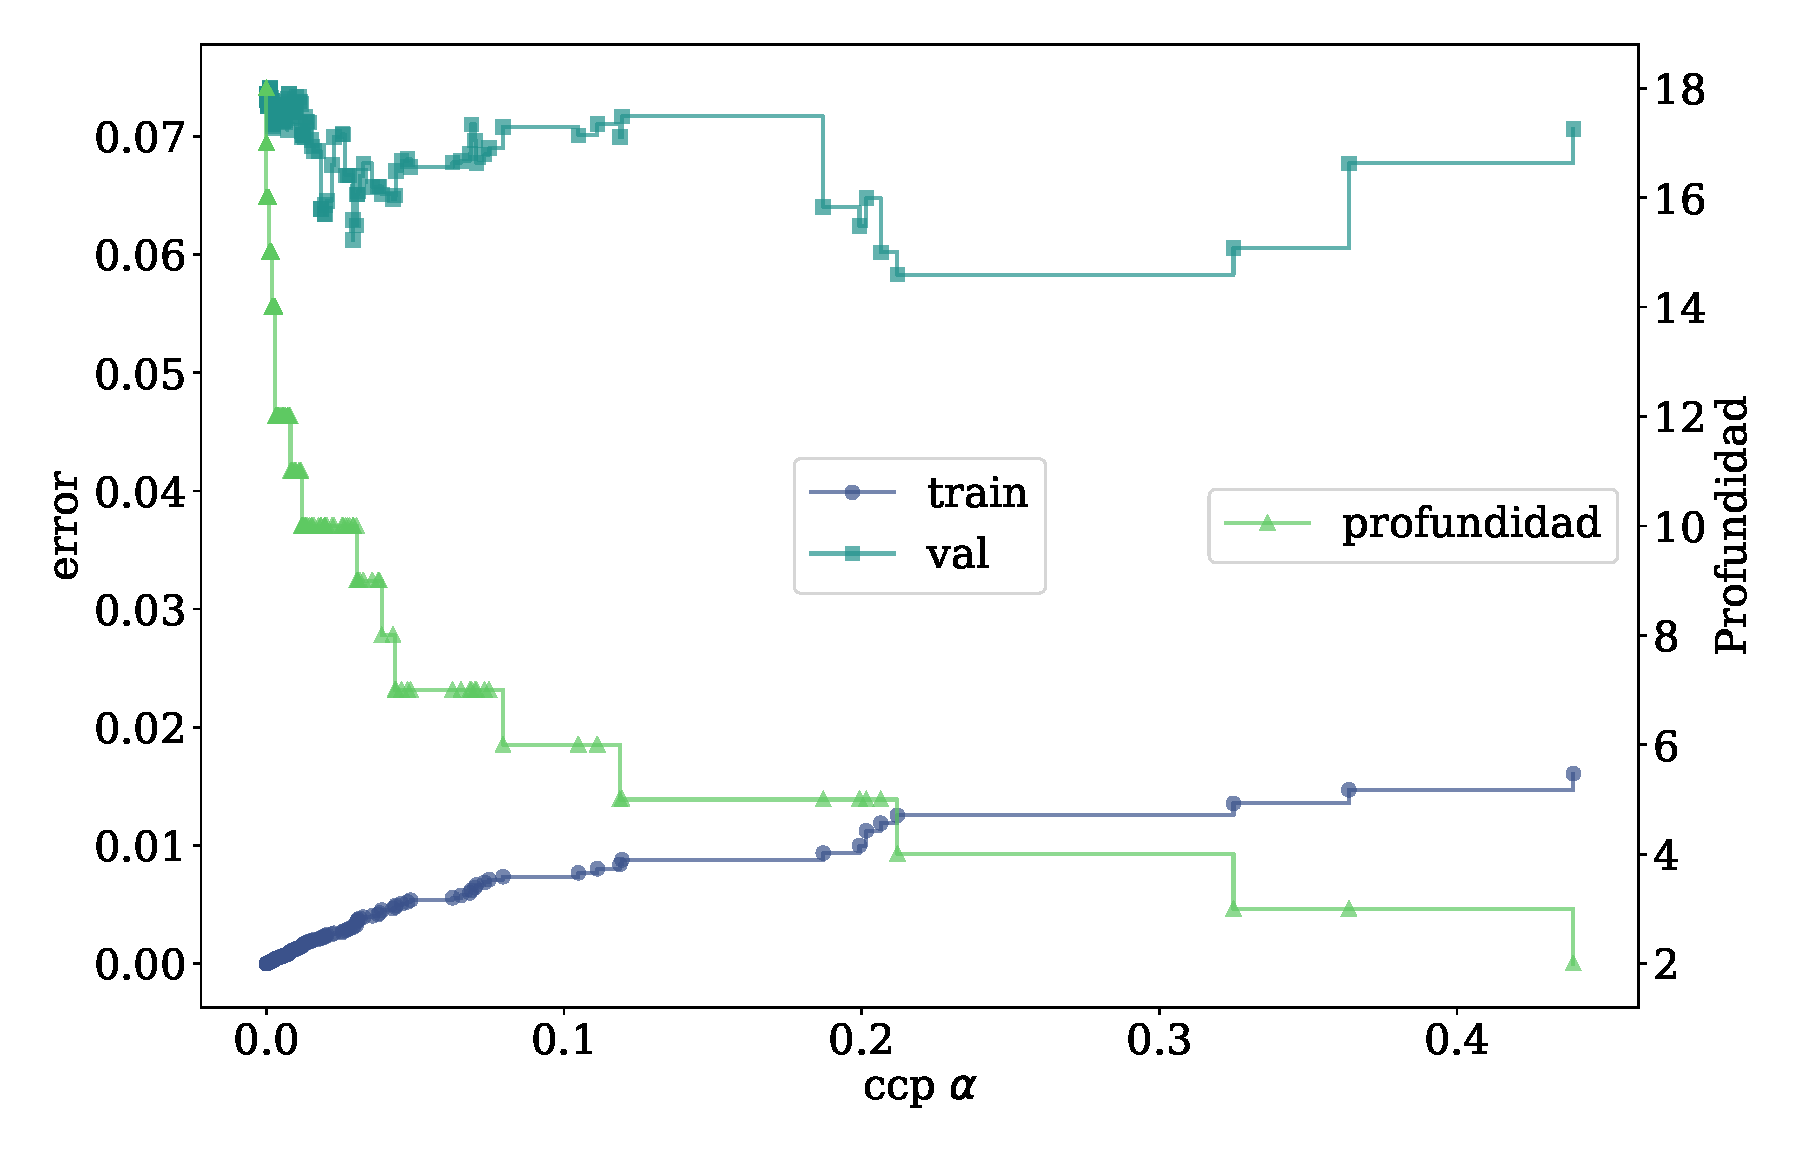
\includegraphics[width=0.5\textwidth]{figures/params_cpp.pdf}
		\end{center}
		\caption{Error y Profundidad de los datos de entrenamiento y error de validación en función del valor de $\alpha_{cpp}$ }
		\label{fig:params_ccp}
	\end{small}
\end{figure}



\subsection*{Item F}
% (f)  Para el caso de regresión,  usar el abordaje tipobaggingpara mejorar el error de test.Comparar con el abordaje de un único árbol de decisión.  Buscar enscikit-learncómo determinar el orden de importancia de los atributos.

En este  item se compararon los resultados del árbol de regresión y un conjunto de árboles de decisión, implementados mediante Bagging. El mismo instancia distintos árboles para varias particiones del conjunto de datos, luego ajusta los parámetros de cada árbol y la función \verb|predict| devuelve la media de las salida de todos los árboles. En este trabajo se optó por usar 25 árboles distintos un Bagging Forest.

Considerando que en el item anterior se obtuvo mediante \verb|GridSearchCV| que el valor óptimo de $\alpha_{cpp}=0.2$, se instanciaron árboles con $\alpha_{cpp}=0.0$ y $\alpha_{cpp}=0.2$ para comparar resultados en las Tablas \ref{tab:item_F_0} y \ref{tab:item_F_2}. En ambas tablas se puede observar que el Bagging tiene una precisión mejor que un sólo árbol ya que el overfitting disminuyó. Otro aspecto es el error de validación, donde un sólo árbol tiene un error mayor que utilizando el emsemble.

%\subsubsection*{Parámetro $\alpha_{cpp}=0$}
\begin{table}[H]
	\begin{small}
		\begin{center}
			\begin{tabular}[c]{l|c|c}
				Atributo	&Simple		&Bagging	\\\hline \hline
				CompPrice   &0.1045		& 0.1148	\\ \hline
				Income      &0.0980		& 0.0706	\\ \hline
				Advertising &0.0413		& 0.0730	\\ \hline
				Population  &0.0429		& 0.0340	\\ \hline
				Price       &0.2960		& 0.2946	\\ \hline
				ShelveLoc   &0.2739		& 0.2932	\\ \hline
				Age         &0.0986		& 0.0840	\\ \hline
				Education   &0.0195		& 0.0279	\\ \hline
				Urban       &0.0151		& 0.0053	\\ \hline
				US          &0.0097		& 0.0022	\\ \hline \hline
				Error de entrenamiento& 0.0&0.0015\\  \hline
				Precisión de entrenamiento & 1 & 0.95 \\ \hline
				Error de validación & 0.07 & 0.03 \\ \hline
				Precisión de validación &0.32 &0.63 \\\hline
			\end{tabular}
		\end{center}
	\end{small}
	\caption{Características de los árboles de regresión posterior al ajuste en el item F con $\alpha_{cpp}=0$}
	\label{tab:item_F_0}
\end{table}

%\subsubsection*{Parámetro $\alpha_{cpp}=0.2$}
\begin{table}[H]
	\begin{small}
		\begin{center}
			\begin{tabular}[c]{l|c|c}
				Atributo	&Simple		& Bagging	\\\hline \hline
				CompPrice   &0.0864		& 0.0634	\\ \hline
				Income      &0.     	& 0.0240	\\ \hline
				Advertising &0.0432		& 0.0771	\\ \hline
				Price       &0.3588		& 0.3269	\\ \hline
				ShelveLoc   &0.4198		& 0.4408	\\ \hline
				Age         &0.0919		& 0.0678	\\ \hline
				\hline
				Error de entrenamiento		& 0.0099& 0.0077\\  \hline
				Precisión de entrenamiento 	& 0.60 	& 0.70 \\ \hline
				Error de validación 		& 0.06 & 0.045 \\ \hline
				Precisión de validación 	& 0.36 	& 0.53 \\\hline
			\end{tabular}
		\end{center}
	\end{small}
	\caption{Características de los árboles de regresión posterior al ajuste en el item F con $\alpha_{cpp}=0.2$}
	\label{tab:item_F_2}
\end{table}


Las importancias ó importancia de gini de cada atributo es número que indica cuan relevantes son esos atributos en la regresión, las mismas son un atributo para la clase del árbol utilizado en \verb|sklearn|. Para obtener las importancias de los atributos en el Bagging, se tomó la media para cada atributo a partir de todos los árboles del emsemble. Con $\alpha_{cpp}=0.0$, el parámetro con mayor importancia para un árbol simple en todas las ejecuciones del código resultó ser el precio del asiento, en cambio para el Bagging el parámetro más importante varía entre ejecución pudiendo ser la posición en la vitrina o el precio del asiento. Con $\alpha_{cpp}=0.2$, como se observa en la Tabla \ref{tab:item_F_2}, hay atributos cuyo peso es nulo, esto se debe a que no son utilizados en la regresión. Además en este caso el atributos con mayor importancia resultó ser la posición en la vitrina del negocio.

Comparando las precisiones sobre la validación en el Bagging con $\alpha_{cpp}=0.0$ y $\alpha_{cpp}=0.2$, se observa en las tablas que el primero llega a una mejor precisión que la segunda opción. Por lo que en el Bagging Forest, se tiene una mejor generalización con $\alpha_{cpp}=0.0$.


% (g)  Usarrandom forestspara mejorar los resultados datos. Comparar el error de test con losabordajes anteriores.  ¿Cambia el orden de la importancia de los atributos?  Hacer unplot con el error de test en función del del hiperparámetromax_featuresque limitael número de atributos a incluir en cada split.  Hacer otro plot equivalente en funcióndemax_depth.1
\subsection*{Item G e Item H}

En este item seguimos abordando el problema de regresionar la cantidad de asientos vendidos con otros datos, utilizando distintos emsembles de árboles de regresión. En las Tabla\,\ref{tab:item_G_H} se comparan las importancias, errores y precisiones para los emsembles Random Forest y AdaBoost. Para realizar los ajustes se tomaron 25 árboles en cada emsemble, sin condiciones en la profundidad y con el valor de $\alpha_{cpp}$ nulo. 

\begin{table}[H]
	\begin{small}
		\begin{center}
			\begin{tabular}[c]{l|c|c}
				Atributo	&Random Forest	& AdaBoost	\\\hline \hline
				CompPrice   &0.1062		& 0.1180	\\ \hline
				Income      &0.0594		& 0.0704	\\ \hline
				Advertising &0.0818		& 0.0793	\\ \hline
				Population  &0.0406		& 0.0340 	\\ \hline
				Price       &0.2778		& 0.2929	\\ \hline
				ShelveLoc   &0.2952		& 0.2902	\\ \hline
				Age         &0.1000		& 0.0773	\\ \hline
				Education   &0.0280		& 0.0274 	\\ \hline
				Urban       &0.0068		& 0.0063 	\\ \hline
				US          &0.0041		& 0.0044 	\\ \hline 
				\hline
				Error de entrenamiento		&0.0013	  &0.0012 \\  \hline
				Precisión de entrenamiento 	& 0.946		&0.953  \\ \hline
				Error de validación 		& 0.0369	&0.0334  \\ \hline
				Precisión de validación 	& 0.621		& 0.656 \\\hline
			\end{tabular}
		\end{center}
	\end{small}
	\caption{Comparación entre los emsembles de regresión Random Forest  y AdaBoost  posterior al ajuste en los items G  y H con $\alpha_{cpp}=0.0$}
	\label{tab:item_G_H}
\end{table}

Comparando  los errores de validación de los árboles de regresión anteriores con los emsembles de este inciso, el Random Forest y el AdaBoost tienen los menores errores en este trabajo, donde el último emsemble es el menor valor obtenido. También el AdaBoost tiene la precisión de validación más alta entre los árboles y emsembles utilizados.

Las importancias de los atributos  del Random Forest, comparado con el Bagging, en cada ejecución la posición en  la vitrina era la más importante, mientras que en el Bagging dependía de la ejecución si la posición o el precio era más importante. Esto varía con los datos tomados en cada fold del k-fold en el Bagging.


En la ejecución de los emsembles de este inciso, se puede definir cual es la profundidad de los árboles del emsembles o cual es la cantidad de atributos considerados para hacer la regresión. En las Figs.\,\ref{fig:params_feat} y \ref{fig:params_prof} se muestran los errores de validación en función de los parámetros mencionados anteriormente.


Para la Fig.\,\ref{fig:params_feat}, se deja libre el parámetro de profundidad de la red. La cantidad de atributo a considerar puede variar entre 1 y 10, dado que la máxima cantidad de atributos disponibles son 10. Los errores varían entre ejecuciones por lo que en la figura mencionada se presenta la media de 10 ejecuciones distintas. Se  observa que hay un mínimo en la curva cuando se toman 5 atributos, y que para el AdaBoost se obtiene el menor error en este valor.

Para la Fig.\ref{fig:params_prof} se varía el parámetro de profundidad mientras que el número de atributos a considerar son 10, que es el predeterminado. Lo mismo que para la figura anterior, se tomó el promedio de 10 ejecuciones. Se observa que para una profundidad a partir de 5 es error permanece constante.

\begin{figure}[H]
	\begin{small}
		\begin{center}
			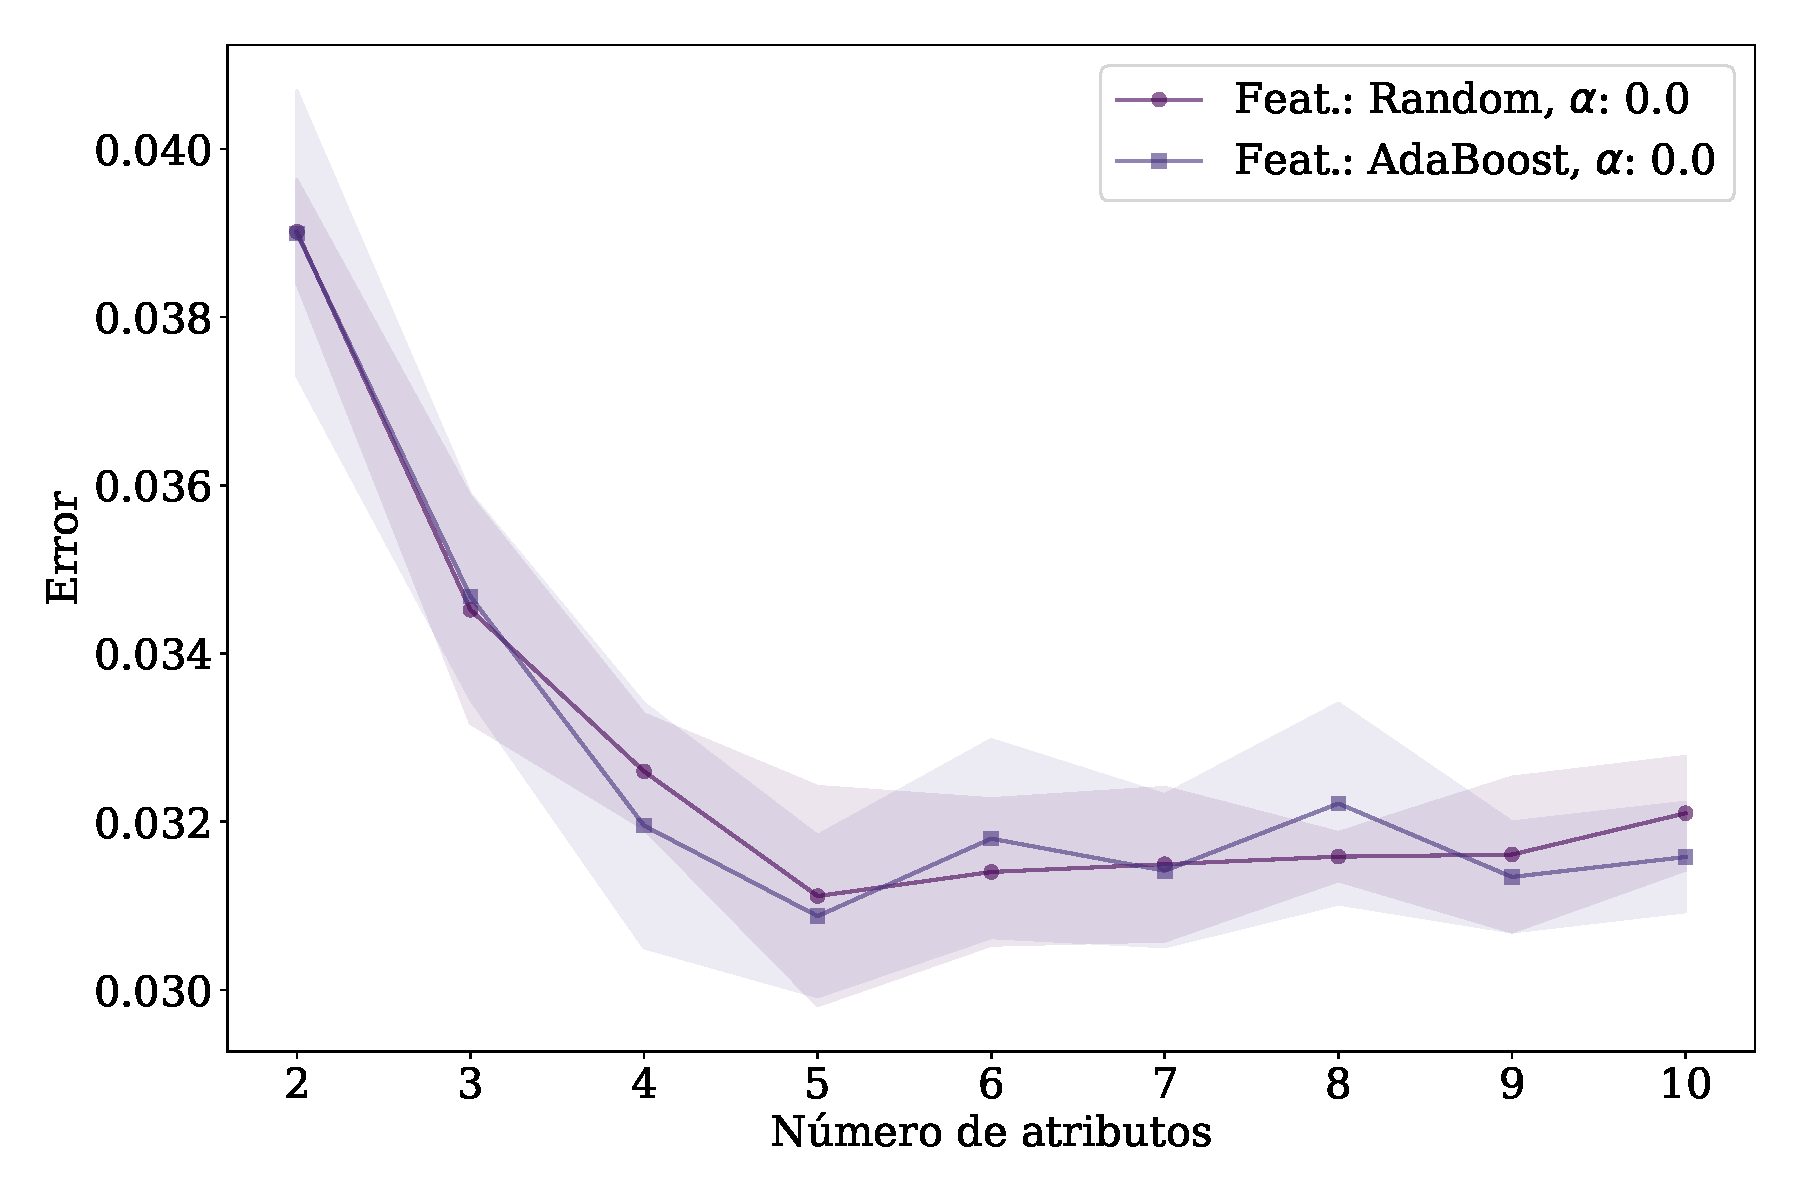
\includegraphics[width=0.5\textwidth]{figures/err_feat_item_gh.pdf}
		\end{center}
		\caption{Error medio de 10 ejecuciones del programa en función del número de atributos para Random Forest y AdaBoost.}
		\label{fig:params_feat}
	\end{small}
\end{figure}

\begin{figure}[H]
	\begin{small}
		\begin{center}
			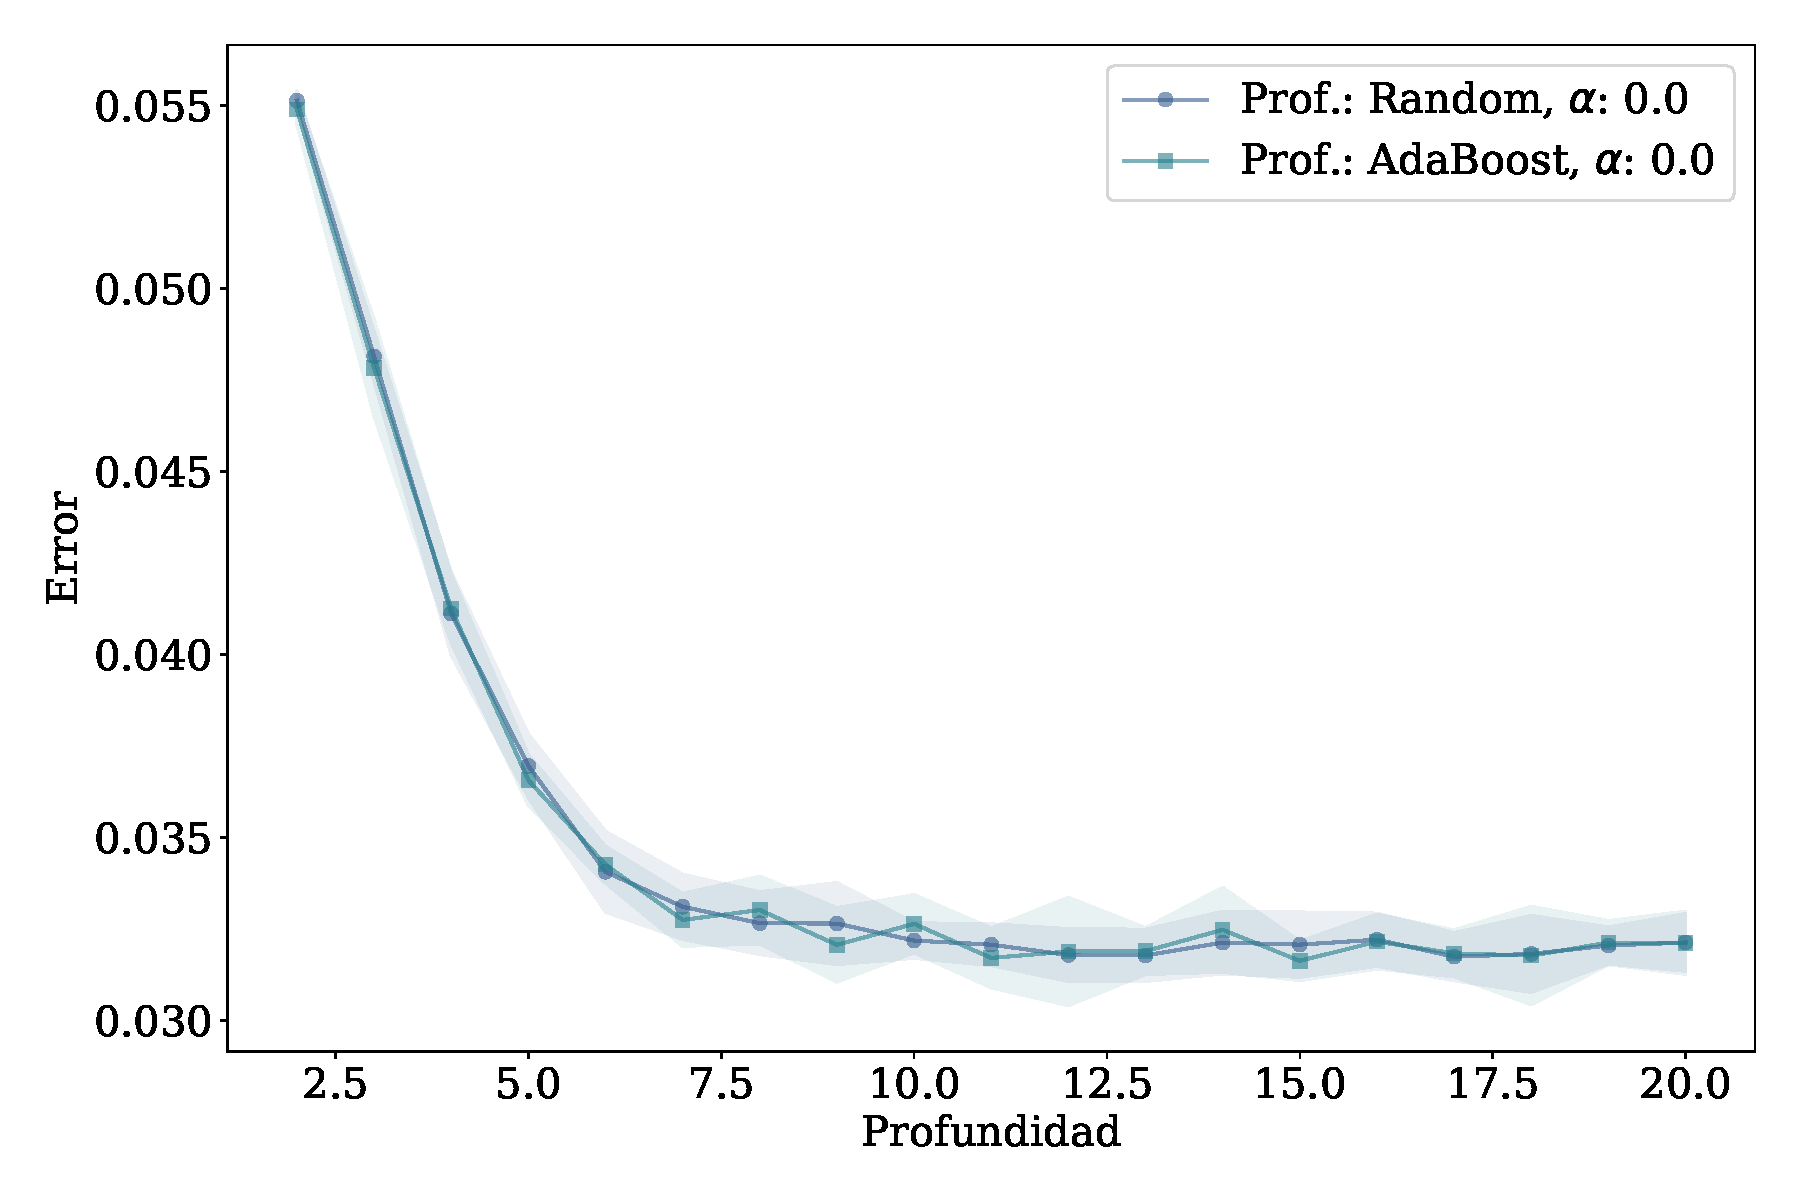
\includegraphics[width=0.5\textwidth]{figures/err_prof_item_gh.pdf}
		\end{center}
		\caption{Error medio de 10 ejecuciones del programa en función de la profundidad de los emsembles Random Forest y AdaBoost.}
		\label{fig:params_prof}
	\end{small}
\end{figure}

\end{document}